\newpage
\chapter{Umsetzung}

\section{Kommunikation}

\subsection{Messages}
Um die Messages sowohl auf dem Server als auf den Android Apps nutzen zu können, müssen alle Messages zu jeder Zeit überall verfügbar sein. Daher wurde ein seperates Projekt angelegt. Es wird jeweils nach MavenLocal deployed um es in den anderen Projekten verfügbar zu machen.

\section{Multicopter Hardware}

Um unsere Plattform testen zu können, haben wir zwei identische Quadcopter aufgebaut.
Wichtig dabei ist, dass für die Benutzung unserer Plattform kein identischer Aufbau nötig ist. Es wird lediglich ein Flight-Controller mit einer MAV-Link kompatiblen Firmware benötigt. z.B. ArduCopter, PX4, usw. 

\subsection{Frame und Antrieb}

Der Frame, die Motoren und ESCs wurden als Kit gekauft. Es handelt sich dabei um ein DJI Flamewheel 450 Frame mit DJI 2312 960kV Motoren und ESeries 420 20A ESCs. Dieses Kit ist weltweit gut verfügbar und deshalb ideal geeignet um einen Versuchsaufbau zu erstellen.

\begin{figure}[h]
	\centering
	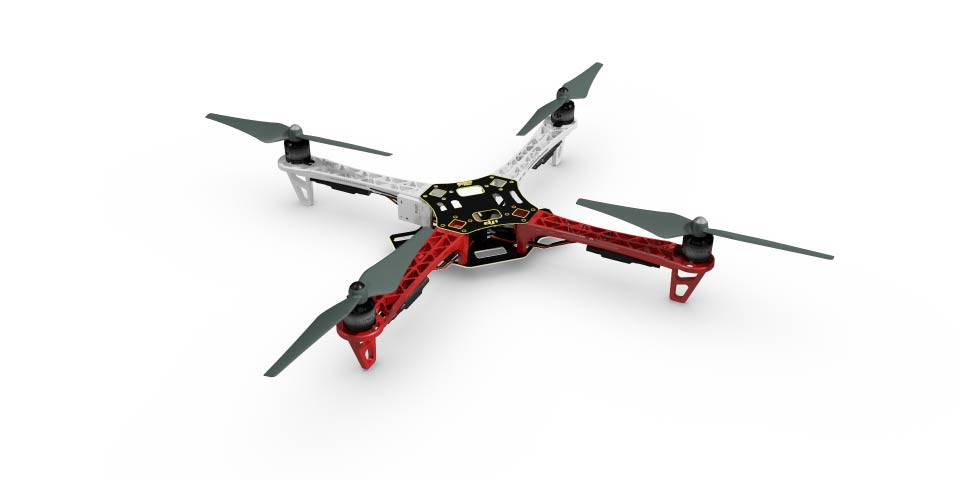
\includegraphics[width=0.9\textwidth] {images/hardware/f450.jpg} 
	\caption{DJI F450 Flamewheel Kit}
	\label{fig:f450}
\end{figure}


\subsection{Flight-Controller}

Der Flight-Controller ist das Herzstück eines Quadcopters. Im Unterschied zu anderen Ferngesteuerten Fahr- und Flugzeugen kann ein Multicopter nur über ein Fly-by-Wire System kontrolliert werden. Das heisst alle Befehle, die von der Fernbedienung kommen, müssen interpretiert und umgewandelt werden, damit die Motoren eine Bewegung in die gewünschte Richtung zu erzeugen können. In Kombination mit einem GPS Modul (Abb. \ref{fig:gps-module}) ermöglich der Controller verschiedene Flugmodi, wie beispielsweise das Schweben an einem Punkt oder automatisches abfliegen von Wegpunkten.

Als Flight-Controller setzen wir ein Pixhawk ein. Es ist sehr vielseitig und kann gut mit zusätzlichen Sensoren erweitert werden, ausserdem unterstützt es gängige Firmwares, die auch auf günstigeren Controllern laufen. Als Firmware für das Pixhawk setzen wir ArduCopter ein, da sie komplett Open-Source ist und auch bei vielen anderen Projekten eingesetzt wird. Sie unterstützt ausserdem das MAV-Link Protokoll, das es ermöglicht verschiedene Hardware über den USB Port anzusprechen.

\begin{figure}[h]
	\centering
	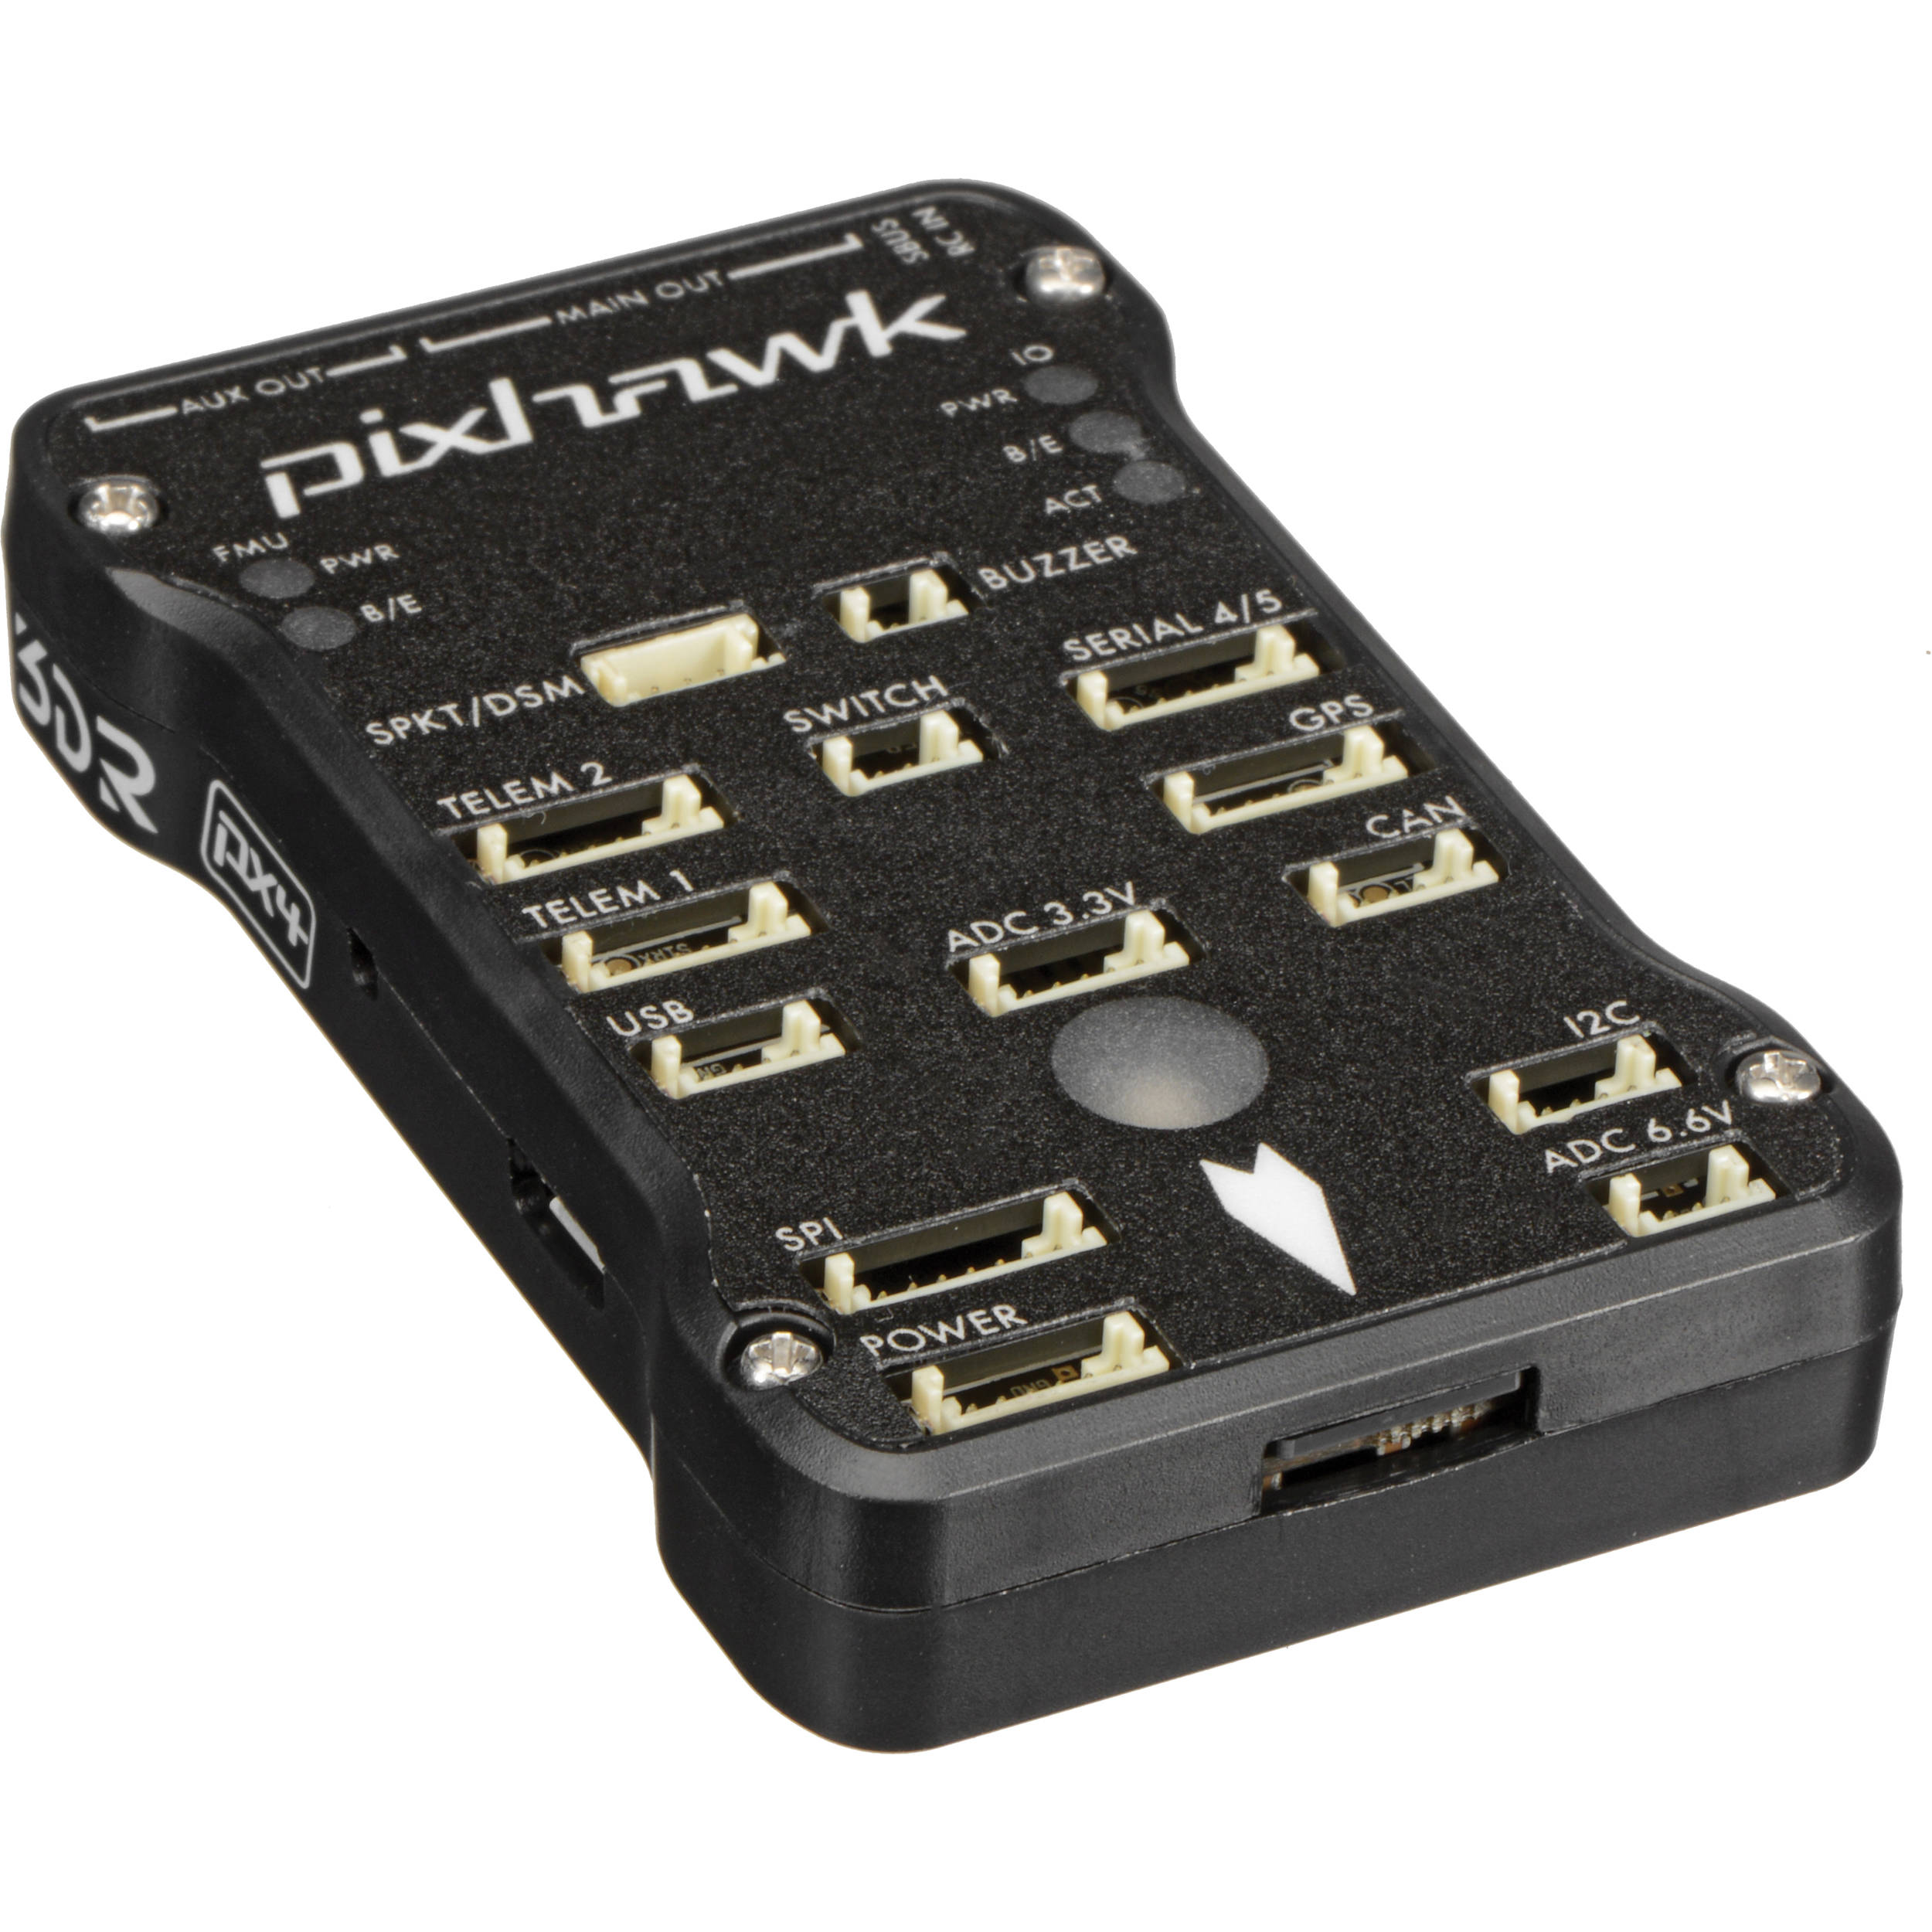
\includegraphics[width=0.3\textwidth] {images/hardware/pixhawk.jpg} 
	\caption{Pixhawk Flight-Controller}
	\label{fig:pixhawk}
\end{figure}

\begin{figure}[h]
	\centering
	
\includegraphics[width=0.3\textwidth] {images/hardware/gps-module.jpg} 
	\caption{GPS-Modul für Pixhawk}
	\label{fig:gps-module}
\end{figure}

\subsection{Ausbaustufen}

Während des Projekts wurden die Hardware laufend den Bedürfnissen angepasst. Daher gibt es mehrere Prototypen, die für die Versuche genutzt wurden.

\subsubsection{Prototyp 1}

Um das Zusammenspiel der Hardwarekomponenten zu testen und erste Versuche mit dem GPS und den verschiedenen Flugmodi zu sammeln, wurde sehr schnell ein Prototyp gebaut.

\begin{figure}[h]
	\centering
	\includegraphics[width=0.9\textwidth] {images/hardware/prototype1.jpg} 
	\caption{Erster Prototyp ohne Landegestellt und ohne Smartphone}
	\label{fig:prototyp-1}
\end{figure}

\subsection{Tests}

Um die Anwendungsmöglichkeiten eines solchen Multicopters auszuloten wurden diverse Experimente durchgeführt um die Leistungsfähigkeit und die Einschränkungen zu testen. 

\subsubsection{Akku Laufzeittest}
Um die maximale Akku Laufzeit zu testen wurde die Drohne ohne zusätzliches Gewicht gestartet, etwa 1.5m über dem Boden schweben gelassen und die Zeit gemessen. Dabei versucht die Drohne die Postion zu halten, bei Abweichung wurde aktiv korrigiert. \\

\begin{tabularx}{\textwidth}{|c|c|X}
    \hline
    \textbf{Akku} & \textbf{Zuladung}  & \textbf{Laufzeit} \\
    3S & keine & 16min 29s\\ \hline 
    2x 4S & 500g & 19min\\ \hline 
\end{tabularx}\\

\subsubsection{Tragfähigkeitstests}

Um das maximale Gewicht zu prüfen, das bei einer Präsentation auf unsere Drohnen geladen werden kann, wurden Tests mit dem Zielgewicht von ca. 500g gemacht.Dies Entspricht dem Gewicht einer PET-Flasche eines beliebigen Getränkeherstellers. Ausserdem war auch das Mobiltelefon (ca. 150g) auch auf der Drohne angebracht.  \\

\begin{tabularx}{\textwidth}{|c|c|c|c|X|}
	\hline
	\textbf{Nutzlast} & \textbf{Akku Typ} & \textbf{Nötige Leistung }& \textbf{Erwartete Flugzeit } & \textbf{Subjektives Flugverhalten }\\
	\hline \hline
	500g & 3S & ca. 75\%  & n.A. & Ziemlich Träge, mehr Gewicht wäre kritisch\\
	\hline
	500g & 4S & ca. 45\%  & n.A. & Gewicht kaum Spürbar\\
	\hline  
\end{tabularx}\\

Auch mit 3S Akkus scheint es also möglich eine PET-Flasche zu transportieren. 

\section{Libraries}

\subsection{Server}


\subsection{Onboard App}
\begin{tabularx}{\textwidth}{|X|X|c|X|}
	\hline
	\textbf{Name} & \textbf{Verwendungszweck} & \textbf{Version} & \textbf{Lizenz} \\
	\hline \hline
	DroneKit-Android Client library & Android API für MAV-Link Protokoll (Ansteuerung der Drohne) & 1.5.1 & Apache 2.0\\
	\hline 
	AMQP Messaging Library & Messaging für Android & 3.6.0 &  Mozilla Public License 1.1, GPL 2,  Apache 2.0 \\
	\hline 
	Lyra  & High availability Messaging & 0.4.3 &  Apache 2.0 \\
	\hline 
\end{tabularx}
\subsection{User App}


\section{Implementierung}

\subsection{Code Standard}
Im Team wurden folgende Code-Conventions eingeführt.

\subsubsection{Kein Author}
In Java wird klassicherweise der Autor im Javadoc Kommentar in der Klasse angegeben.

\begin{lstlisting}
/**
 * @author Kirusanth Poopalasingam (pkirusanth@gmail.com)
 */
public class MyTestClass{
}
\end{lstlisting}

Der Autor in der Klasse suggeriert, dass nur ein Autor für diese Klasse existiert und für diese Klasse zuständig ist. Dies ist aber meist nicht der Fall. 
Der Code sollte von allen Teammitgliedern gepflegt werden. Ausserdem ist die Angabe auf der Klasse heutzutage mit einem Version Control System redundant.

\subsubsection{Javadoc}
Generell sollte Javadoc nur dort verwendet werden, wo es nötig ist. Da es sich beim Helin Projekt nicht um eine API handelt, sollten auch die Methoden und Parameter nicht redundant dokumentiert werden. Ein Beispiel für eine schlechte Javadoc Dokumentation sieht folgendermassen aus :

\begin{lstlisting}
// Beispiel einer Play Klasse
public final class ConfigUtil {
    private ConfigUtil() { }

    /**
     * Quotes and escapes a string, as in the JSON specification.
     *
     * @param s
     *            a string
     * @return the string quoted and escaped
     */
    public static String quoteString(String s) {
        return ConfigImplUtil.renderJsonString(s);
    }
    // ...
}
\end{lstlisting}

Bei der Methode quoteString() kann der ganze JavaDoc weggelassen werden, da er nicht mehr aussagend ist, als die Methode selbst.
Stattdessen sollte die Methode so geschreiben werden, dass die Namen aussagekräftiger sind.

Besser wäre:
\begin{lstlisting}
public final class ConfigUtil {
    private ConfigUtil() { }

    public static String quoteStringAccordingToJsonSpecification(String unquotedJson) {
        return ConfigImplUtil.renderJsonString(unquotedJson);
    }
    // ...
}
\end{lstlisting}

\subsubsection{Code}
Für die Formattierung und den Static Check werden die Inspections von IntelliJ IDEA verwendet.
Diese sind konfigurierbare Regeln, welche mit dem Projekt eingecheckt werden. Der IDE führt diese vor dem einchecken aus und verhindert das einchecken falls diese Verletzten werden.
Da es zu viele von den Regeln zur Verfügung stehen, wurde die Vorlage von IntelliJ genommen und ins VCS eingecheckt, damit alle diesselben Regeln verwenden.

\subsection{Messaging}

Um die nichtfunktionalen Anforderungen im Bereich der Kommunikation zu erfüllen, wurde AMQP als Protokoll ausgewählt. Mit Messaging soll gewährleistet werden, dass die Verbindungswiederherstellung funktioniert. Die funktionale Anforderung des Missionsabbruchs wird somit soweit gedeckt, dass versucht wird die Verbindung aufrechtzuerhalten, sofern das Netz es erlaubt. Bei kurzen Netzunterbrüchen kann somit über das AMQP Protokoll eine Verbindung zur Drohne gewährleistet werden.

\begin{itemize}
	\item{\textbf{Verbindungsabbruch:} \\
	Gemäss den nicht funktionalen Anforderungen darf der Verbindungsabbruch keinen Einfluss auf die Mission haben. Um gemäss den funktionalen Anforderungen einen Missionsabbruch zu gewährleisten, wird versucht Unterbrüche so kurz wie möglich zu halten und einen automatischen Verbiundungsaufbau zu ermöglichen. Aus diesem Faktoren wird die gesamte Mission vor dem Start übertragen, damit sie ausgeführt werden kann. Einzelne Wegpunke sind somit nicht auf eine stabile Internetverbindung angewiesen, da die Route bereits von Anfang bekannt ist. Der Missionsabbruch ist ebenfalls gewährleistet - sofern die GSM Verbindung besteht. 
	\\
	Verbindungsabbrüche auf dem Mobiltelefon haben zweierlei Konsequenzen:	
	\begin{itemize}
		\item{\textbf{Mobiltelefon kann die Messages vom Server nicht empfangen:} \\
		Dieses Szenario wird durch das RabbitMQ abgefangen. Der Messaging Broker cached die Nachrichten solange bis der Consumer (Mobiltelefon) wieder verfügbar ist. Es besteht somit kein zusätzlicher Handlungsbedarf auf dem Onboard-App.
		}
		\item{\textbf{Messages vom Mobiltelefon zum Server können nicht gesendet werden:} \\
		In diesem Fall kann der Übertragungsfehler nicht durch RabbitMQ abgefangen werden. Der Broker hat vom Producer (Mobiletelefon) noch keine Nachricht bekommen. Aus diesem Grund wird producerseitig eine Exception geworfen, die darauf hinweist, dass die Verbindung unterbrochen ist. In diesem Fall wird die Nachricht in einem Queue zwischengespeichert. Sämtliche Folgenachrichten, die während des Verbindungsunterbruchs nicht übertragen werden können, werden ebenfalls in dieser Queue gespeichert. Sobald die Verbindung wieder besteht, werden die Nachrichten aus der Queue gesendet.
		}
	\end{itemize}
	Mit diesen Massnahmen ist ein guter Kompromiss aus Zuverlässigkeit und Aufwand entstanden. Alle missionskritischen Nachrichten können übertragen werden. Telemetriedaten sind von einem Verbindungsausfall ebenfalls nicht betroffen.
	}
	\item{\textbf{Verbindungswiederherstellung:}
	Aus den nicht funktionalen Anforderungen ist zu entnehmen, dass bei einem Verbindungsunterbruch ein Reconnect statt findet. Dieser Reconnect soll, sobald die Verbindung im GSM Netz wieder besteht nicht länger als 30s dauern. \\
	Bei der Konfiguration von AMQP bestanden mehrere Möglichkeiten. Einersetis war der bekannte Backoff Algorithmus eine Option. Dieser Algorithmus arbeitet nach einem incrementellen Prinzip. Je länger der Unterbruch dauert, desto länger dauert es bis er die Verbindung wieder versucht aufzubauen. Auf der anderen Seite stand ein einfacher Interval-Algorithmus. Dieser versucht alle drei Sekunden die Verbindung wiederherzustellen, bis zum erfolgreichen Verbindungsaufbau. Mit diesen Erkenntnissen haben wir folgende Messung gemacht:
	\begin{center}
		\begin{tabular}{|r|r|}
		\hline
		  \textbf{Backoff} & \textbf{Interval 3s} \\
		\hline
		  17 & 7 \\
		  7 & 7 \\
		  9 & 7 \\
		  11 & 7 \\
		  10 & 7 \\
		\hline
		% TODO: Kommentar noch: Anzahl Sekunden bis zum Verbindungsaufbau
		\end{tabular}
	\end{center}
	Aus diesen Erkenntnissen standen beide Möglichkeiten offen, denn beide erfüllen die Anforderungen und haben somit auch keine Auswirkungen auf die Qualität. Am Ende wurde bewusst auf den BackOff Algorithmus gesetzt. Der Backoff Algorithmus benötigt zwar deutlich länger für einen Reconnect als das fixe Zeitinterval. Die hetrogene Verteilung der Wiederverbindungszeiten spricht aber für den Backoff Algorithmus. Sollte es zu Probleme auf der Serverseite kommen, so werden nicht alle Geräte gleichzeitig einen Reconnect probieren - der Reconnect passiert somit gestaffelt. Dies bringt zusätzlich Stabilität ins System.}
	\item{\textbf{Android Process Lifecycle:} \\
	Da die OnboardApp auf einem Android Betriebssystem läuft, mussten gewisse Voraussetzungen geprüft werden. Im Grund kann davon ausgegangen werden, dass die Applikation immer im Vordergrund steht. Es ist doch sehr unwahrscheinlich, dass die Appliaktion in den Hintergrund rückt, weil eine andere Applikation verwendet wird. \\
	% TODO Quelle: http://developer.android.com/guide/components/processes-and-threads.html
	Laut Android Dokumentation ist das Verhalten einer Applikation im Hintergrund nicht deterministisch. Sollte eine Applikation im Hintergrund gewisse Garantien haben, so muss von einem Service und der spezifischen Implementierung eines Services gesprochen werden. Im Fall der OnboardApp und den getroffenen Annahmen, wurde davon abgesehen, da die Applikation während des Fluges nicht gewechselt wird.
	}

\end{itemize}